\section{System Overview}

\indent The overview of the system has been described in~\ref{fig:Overview}. The system has two major components - Complete Camera Module and the Image Processing Unit. The Complete Camera Module (CCM) consists of the IR camera, Digital camera and the Motor modules. All three modules are controlled by a Raspberry Pi. The motor rotates by a pre-calibrated angle and both the digital and infrared images are taken simultaneously and sent over to a PC where the Image Processing Unit (IPU) is present. The first task of IPU is pre-processing images and generate the heat maps for the thermal data. In the training phase the digital images are stitched together and the same stitching mechanism is applied for the IR images in testing phase. Processed images give the thermal layout of a wall surface which can be used for analytics.

\begin{figure}[!h]
\begin{center}
	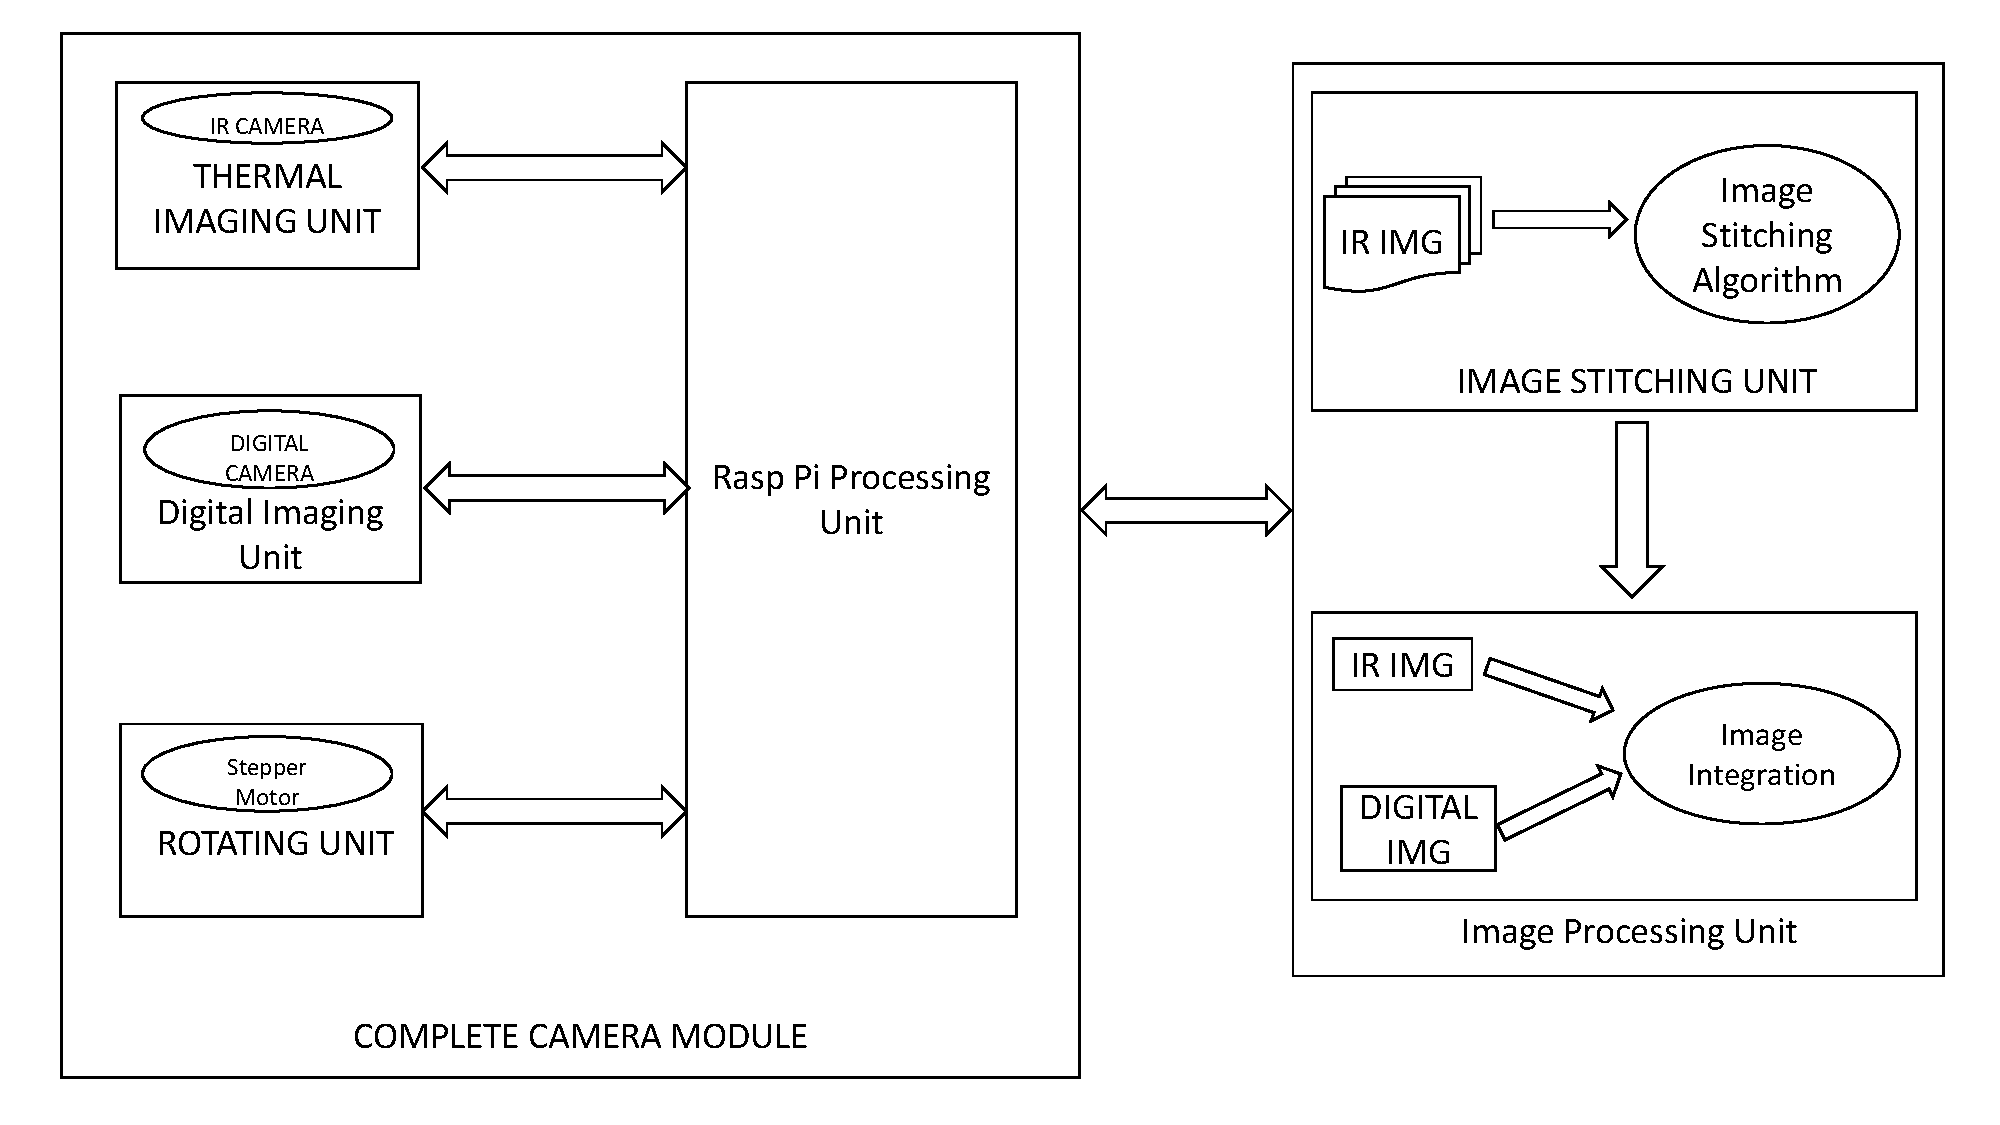
\includegraphics[width=2.5in]{figs/SystemBlockDIagram.pdf}
\end{center}
  \caption{Thermal Imaging System Block Diagram}
  \label{fig:Overview}
\end{figure}
